\documentclass[11pt,french,a4paper]{article}
\usepackage[utf8]{inputenc}
\usepackage[french]{babel}
\usepackage[T1]{fontenc}
\usepackage{fancyhdr}
\usepackage{lastpage}
\usepackage{fancybox}
\usepackage{graphicx}
\usepackage{appendix}
\usepackage[left=2cm,right=2cm,top=2cm,bottom=2.5cm]{geometry}
\geometry{a4paper}
\setlength{\parindent}{0pt}
\usepackage{listings}
\usepackage{color}
\usepackage[table]{xcolor}
\usepackage{array}
\usepackage{listings}
\usepackage{hyperref}
\usepackage{caption}
\usepackage{lastpage}
\pagestyle{fancy}

\definecolor{darkWhite}{rgb}{0.94,0.94,0.94}

\lstset{
  aboveskip=3mm,
  belowskip=-2mm,
  backgroundcolor=\color{darkWhite},
  basicstyle=\footnotesize,
  breakatwhitespace=false,
  breaklines=true,
  captionpos=b,
  commentstyle=\color{red},
  deletekeywords={...},
  escapeinside={\%*}{*)},
  extendedchars=true,
  framexleftmargin=16pt,
  framextopmargin=3pt,
  framexbottommargin=6pt,
  frame=tb,
  keepspaces=true,
  keywordstyle=\color{blue},
  language=C,
  literate=
  {²}{{\textsuperscript{2}}}1
  {⁴}{{\textsuperscript{4}}}1
  {⁶}{{\textsuperscript{6}}}1
  {⁸}{{\textsuperscript{8}}}1
  {€}{{\euro{}}}1
  {é}{{\'e}}1
  {è}{{\`{e}}}1
  {ê}{{\^{e}}}1
  {ë}{{\¨{e}}}1
  {É}{{\'{E}}}1
  {Ê}{{\^{E}}}1
  {û}{{\^{u}}}1
  {ù}{{\`{u}}}1
  {â}{{\^{a}}}1
  {à}{{\`{a}}}1
  {á}{{\'{a}}}1
  {ã}{{\~{a}}}1
  {Á}{{\'{A}}}1
  {Â}{{\^{A}}}1
  {Ã}{{\~{A}}}1
  {ç}{{\c{c}}}1
  {Ç}{{\c{C}}}1
  {õ}{{\~{o}}}1
  {ó}{{\'{o}}}1
  {ô}{{\^{o}}}1
  {Õ}{{\~{O}}}1
  {Ó}{{\'{O}}}1
  {Ô}{{\^{O}}}1
  {î}{{\^{i}}}1
  {Î}{{\^{I}}}1
  {í}{{\'{i}}}1
  {Í}{{\~{Í}}}1,
  morekeywords={*,...},
  numbers=left,
  numbersep=10pt,
  numberstyle=\tiny\color{black},
  rulecolor=\color{black},
  showspaces=false,
  showstringspaces=false,
  showtabs=false,
  stepnumber=1,
  stringstyle=\color{gray},
  tabsize=4,
  title=\lstname,
}


\fancyhead[L]{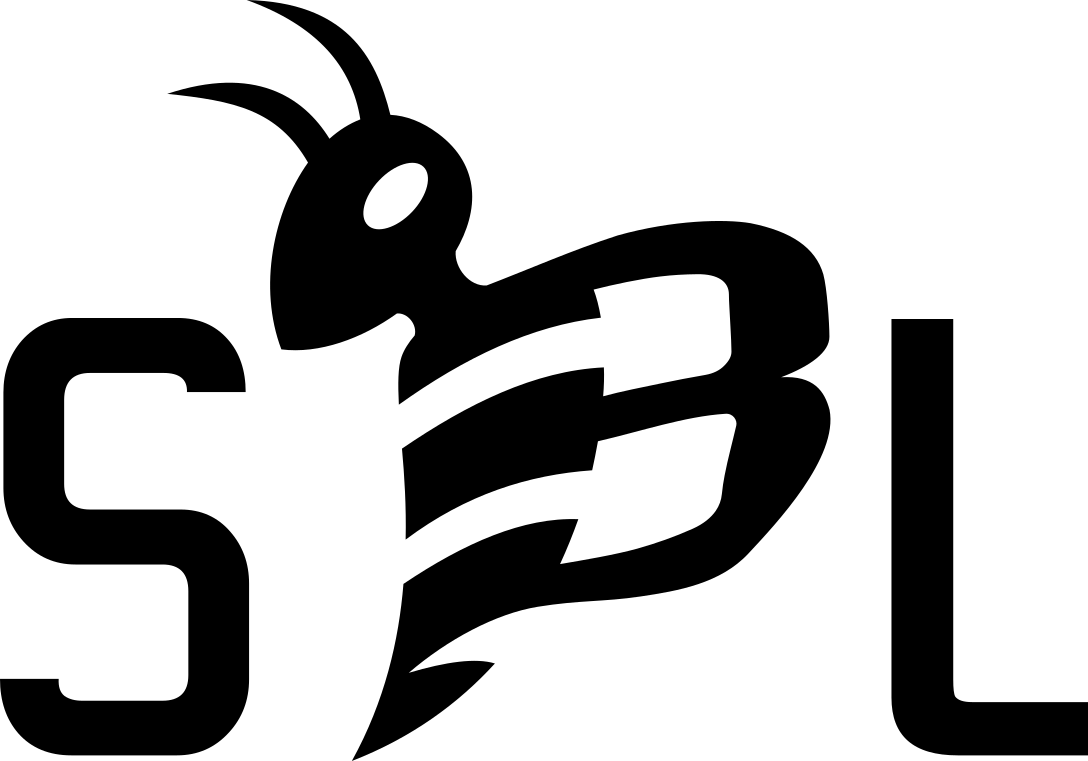
\includegraphics[width=1cm]{../../../logo/SBLlogo.png}}
\fancyhead[C]{Rapport d'activités semaines du 11 et 18 avril 2022 }
\fancyhead[R]{ 
\includegraphics[width=1.2cm]{../../../logo/IUTlogo.png}}
\fancyfoot[L]{\small Tom TUELEAU\normalsize}
\fancyfoot[C]{}
\fancyfoot[R]{\thepage/\pageref{LastPage}}


\lstset{
  basicstyle=\fontfamily{lmvtt}\selectfont\small,
  columns=fullflexible,
}

\title{
 \centering
         
\includegraphics[width=4cm]{../../../logo/IUTlogo.png}  \hspace{7cm}
         
\includegraphics[width=4cm]{../../../logo/UMlogo.png}  \hspace{7cm}
    
	\LARGE{Rapport d'activités des semaines du 9 au 20 mai 2022 }
	\author{TUELEAU Tom}
}
\author{
	\date{}
}
\begin{document}
\maketitle
	 
\includegraphics[width=4cm]{../../../logo/LIRMMlogo.png}  \hspace{7cm}
         \includegraphics[width=4cm]{../../../logo/IBMMlogo.jpg}  \hspace{7cm}
\newpage
\tableofcontents
\newpage
\section{Introduction}
Ce document a pour objectif de faire un état d'avancement du stage. Celui-ci résumera donc le travail fait lors de la fin du mois d'avril et la premier moitié du mois de mai.
\\Dans un premier temps, je reviendrait sur le montage amplificateur vue lors du dernier rapport et vous montrerait les résultats obtenue.
\\Une seconde partie présentera les programmes crée afin de récolter et traiter les données des capteurs. 
\\Une troisième partie traitera de l'envoie des données entre les différents élément du système.
\\Enfin, je conclurait sur le travail effectuer et les difficultés rencontrer. 

\section{Finalisation du montage}
Lors des précédents rapport\footnote{Voir "Rapport d’activités du 11 et 18 avril 2022", partie 4, page 7}, je vous ai exposer mes recherches et résultats quand au dimensionnement d'un montage amplificateur. Ce besoins c'était fait ressentir quand je m'était rendue compte que le signal émis par le piézo-électrique n'arrivait pas à être capter par l'Arduino.  Dans cette partie nous verrons tout d'abords la finalisation du montage et dans un second temps nous verrons l'installation de celui-ci dans le rucher.\\
\subsection{Montage}
Lors de cette semaine j'ai pu effectuer le prototype final incluant l'amplification du signal, le piézo-électrique, le capteur de température et d'humidité (Si7021) et l'Arduino. Vous pouvez voire un schéma complet Figure \ref{SMG}.
\\
\begin{center}
    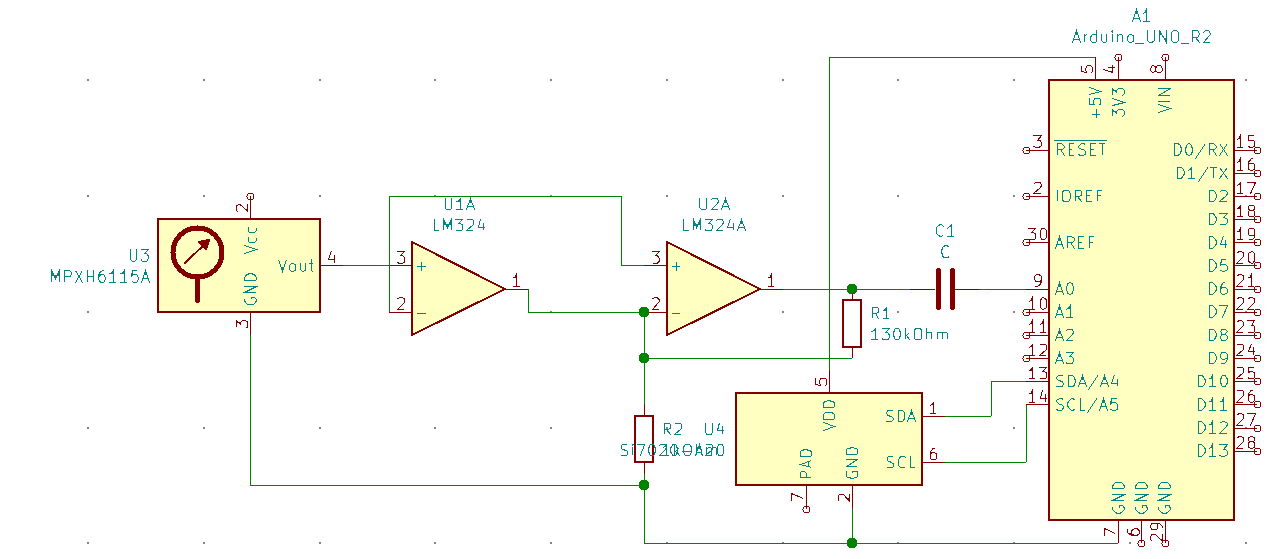
\includegraphics[scale=0.5]{../img/SMG.png}
    \captionof{figure}{Schéma montage final}
    \label{SMG}
\end{center}
Comme nous le verrons lors de la partie programmation, j'arrive à récupérer le signal envoyer par le piézo-électrique avec l'Arduino. Cella vas donc me permettre d'échantillonner celui-ci et de le traiter.
\subsection{Installation dans la ruche}
L'objectif étant de récolter les données dans la ruche, j'ai du installer les capteurs dans celle-ci. Comme vous pouvez le voire Figure \ref{RC}, j'ai glisser les différent capteur dans la ruche et leur ai souder des files assez long pour les brancher par la suite sur un microcontrôleur.

\begin{center}
    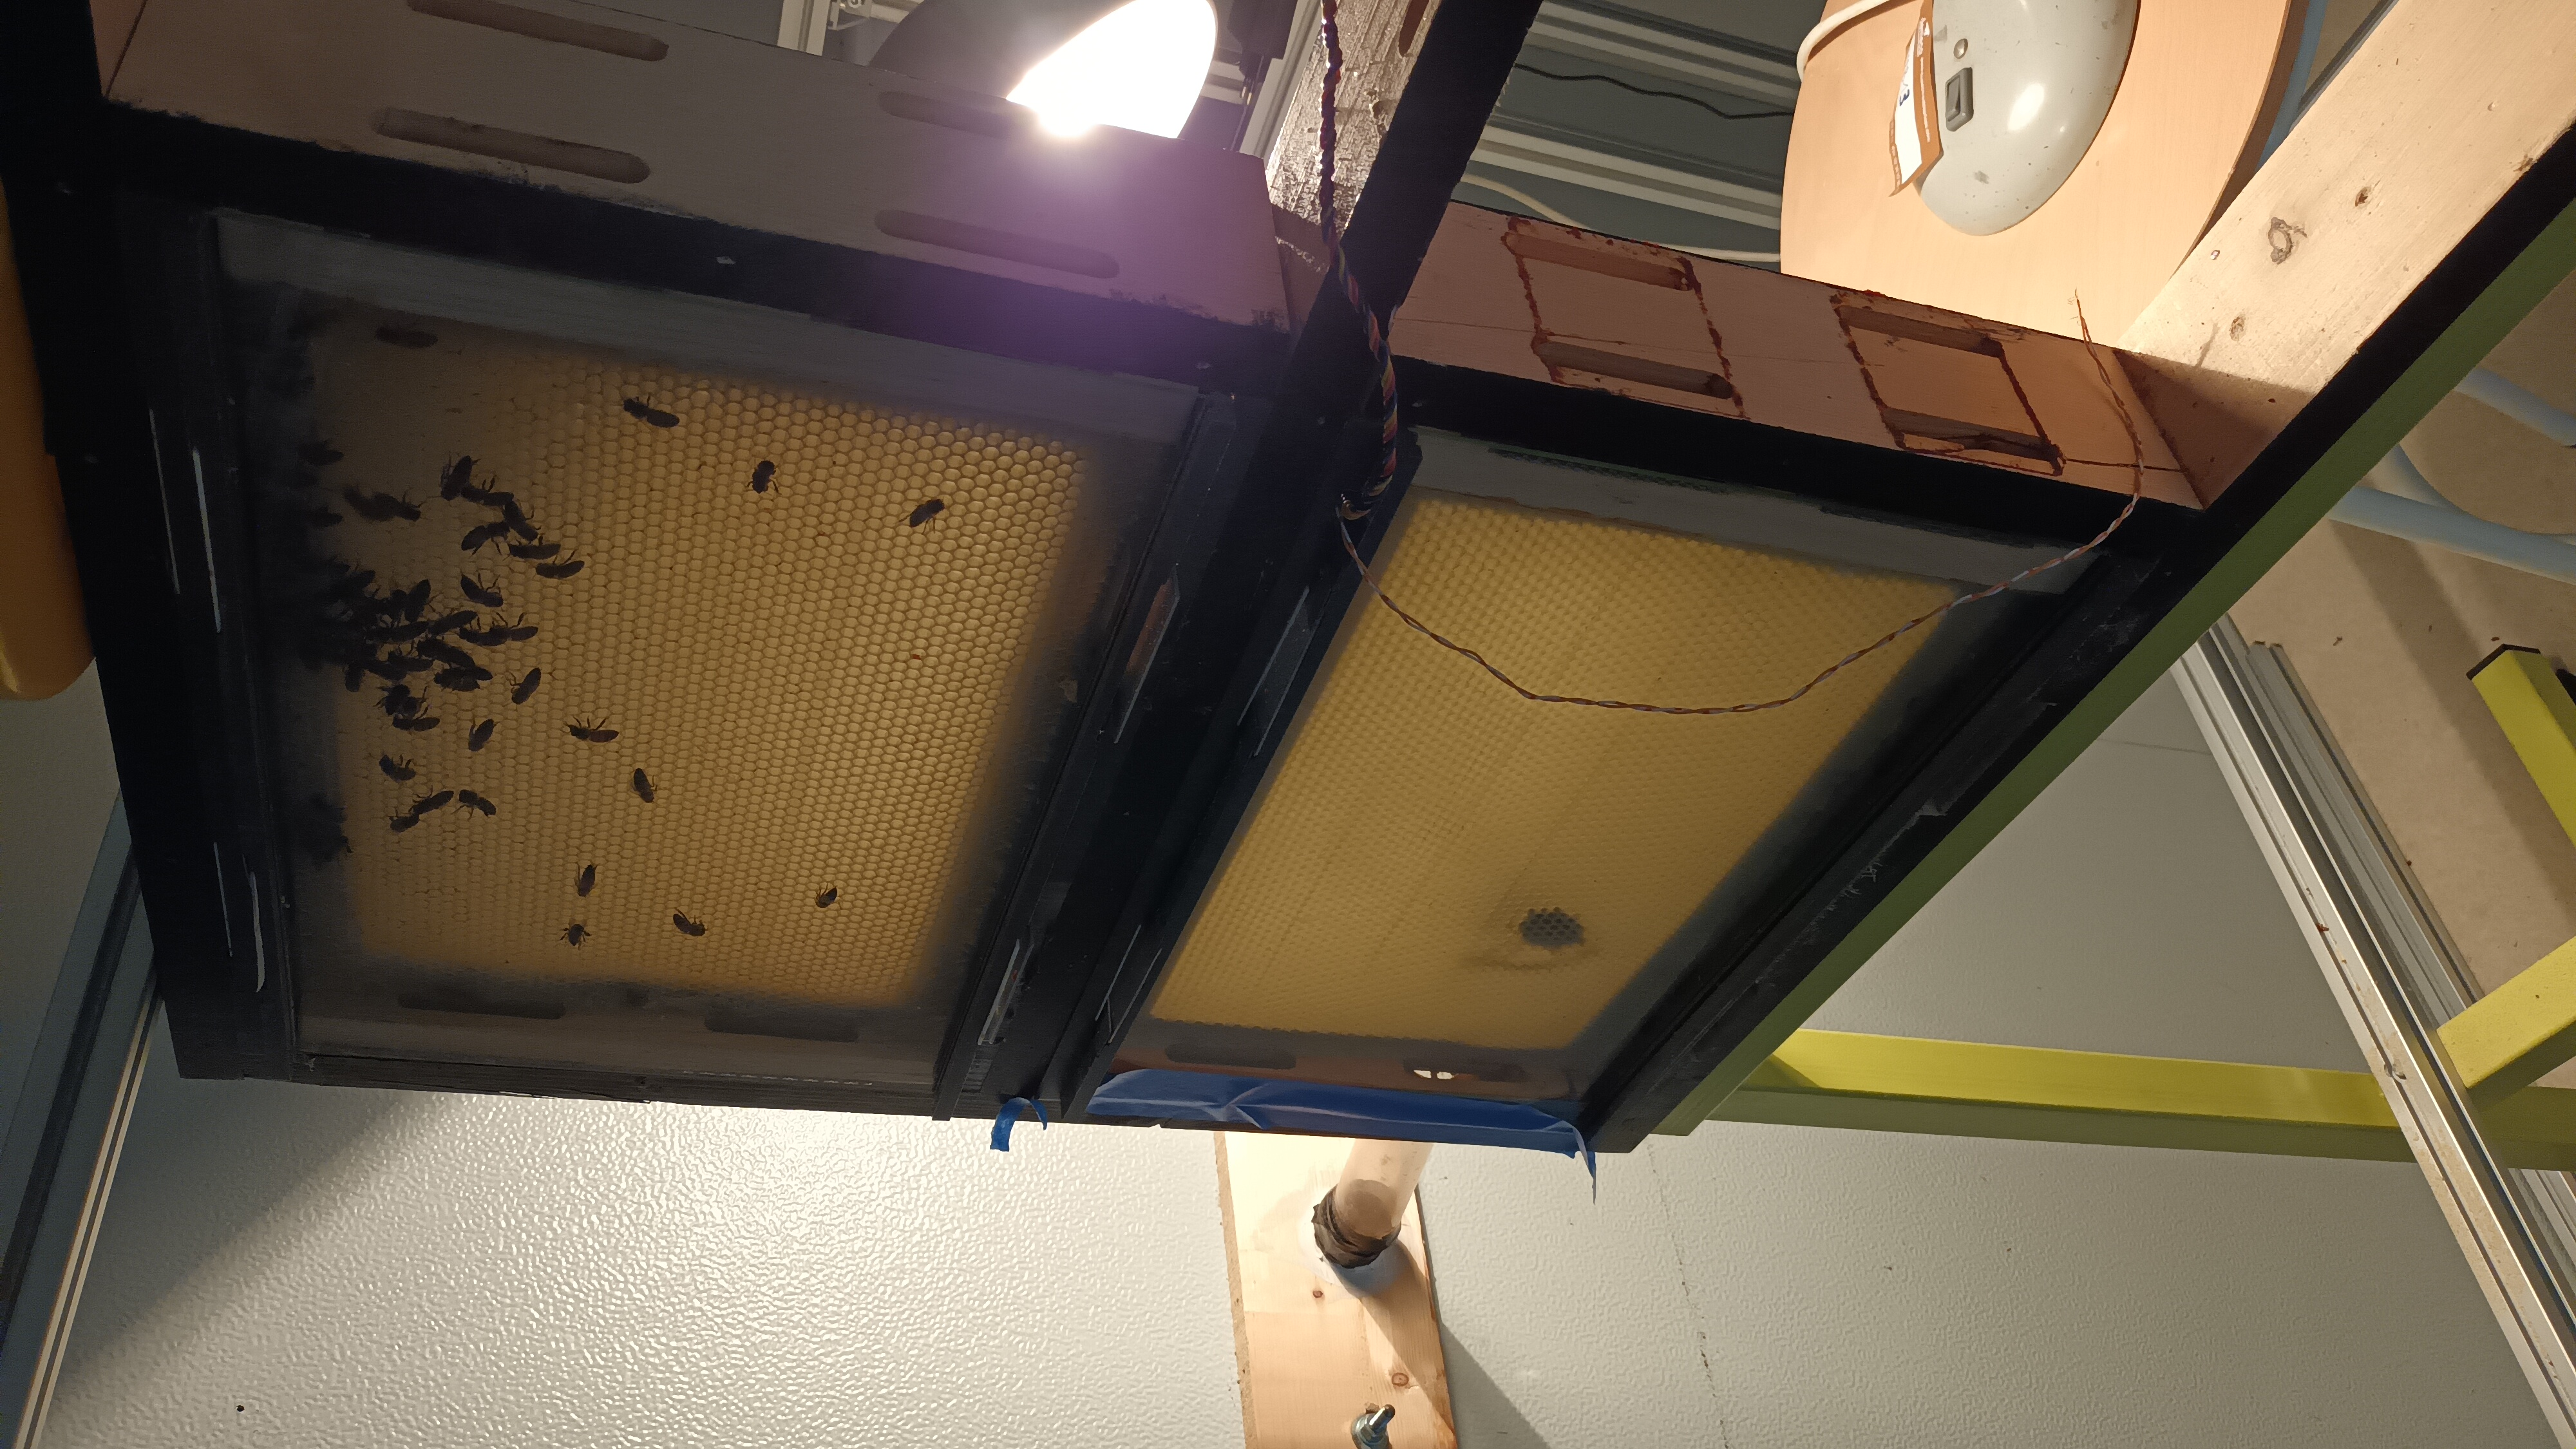
\includegraphics[scale=0.1,angle=270]{../img/RC.png}
    \captionof{figure}{Capteurs dans la ruche}
    \label{RC}
\end{center}
\subsection{Amélioration}
Maintenant que ce montage est fonctionnel, j'aimerais pouvoir lui apporter des améliorations. La première serai la création d'un PCB pour le montage amplificateur afin de rendre le montage plus professionnel. La seconde serait la création d'un boitier pouvant le contenir lui et l'Arduino. 
\newpage
\section{Programmation}
Tout aux long des dernier semaine, j'ai eux à programmer plusieurs fonctionnalité. Dans cette partie je vais donc commencer par vous présenter les programme effectuer pour récolter les données des capteurs et effectuer leur traitement. Une deuxième partie abordera la programmation de la mise en communication des différents composant du système.
\subsection{Programmation des capteurs}
Pour ma premier mission j'avais trois  données à récupérer. Celle-ci sont l'humidité, la température et les vibration. Afin de récolter ces données j'ai choisi en tout trois capteur Un capteur piézo-électrique , un capteur de température et d'humidité (Si7021) et un microphone (INMP441). Dans un premier temps je vous parlerait du capteur de température et d'humidité. Une seconde partie abordera la programmation du capteur de vibration. Enfin une dernier partie abordera le traitement des données.  

\subsubsection{Capteur de température et humidité}
Comme indiquer précédemment le capteur utiliser pour ces données est le Si7021. Étant données que le microcontroleur que j'utilise est un arduino, il existe des librairies donnant accès à des fonction permettant d'obtenir les données voulus.
\begin{scriptsize}
	\begin{lstlisting}
#include <Adafruit_Si7021.h>

Adafruit_Si7021 sensor = Adafruit_Si7021();

void callback(char* topic, byte* payload, unsigned int length) {}

void setup() {
   Serial.begin(9600);
 if (!sensor.begin()) {
    Serial.println("Did not find Si7021 sensor!");
    while (true)
      ;
  }
}

void loop() {
  double hum,temp;
  char Ctemp[4], Chum[4];
  hum = sensor.readHumidity();
  temp = sensor.readTemperature();
  dtostrf(temp,2,2,Ctemp);
  dtostrf(hum,2,2,Chum);
 delay(1000);
}	
	\end{lstlisting}
\end{scriptsize}

Les fonction principals de ce programme sont , "sensor.begin" qui initialise la liaisons entre l'Arduino et le capteur, readHumidity et readTemperature permet comme leurs nom l'indique de récupérer la température et l'humidité messurer par le capteur. Les valeurs retourner par ces deux fonction sont de type "double". Afin de pouvoire les envoyer, je les convertis en chaine de caractère à l'aide de la fonction "dtostrf".

\subsubsection{Capteur de vibration}
Après avoir amplifier le signal du piézo-électrique, j'ai pu me consacrer à l'acquisition des données de cellui-ci. Afin de faciliter sont acquisition j'ai créée une fonction "udpSendVibration" prenant la quantiter d'échantillon souhaités, le nombre de decimal et la pęriode d'échantillonage (en milli seconde).
\begin{scriptsize}
\begin{lstlisting}

void udpSendVibration(int nbEchantillon, int nbVirgule, int periodeEchantillonageMs)
{

	int nbChar = nbVirgule+2;
	char tmp[nbEchantillon][nbChar];
	char data2[nbEchantillon*nbChar];
	double centsValeurs[nbEchantillon];
	int i,y;
	for(i=0;i<nbEchantillon;i++){
		centsValeurs[i]=analogRead(piezo);
		centsValeurs[i]=(centsValeurs[i]*5)/1023;
		delay(periodeEchantillonageMs);
	}
	delay(2000);
	for(i=0;i<nbEchantillon;i++){
		dtostrf(centsValeurs[i],nbChar,nbVirgule,tmp[i]);
		for(y=0;y<nbChar;y++){
			data2[(nbChar*i)+y]=tmp[i][y];
			Serial.println(data2[(i*nbChar)+y]);	
		}	
	}

}
\end{lstlisting}
\end{scriptsize} 

\subsubsection{Traitement des données}
Une fois le signal obtenue il fallait l'annalyser en fréquence. Pour cella j'était dans un premier temps partie pour traiter directement sur l'Arduino en effectuant une transformer de Fourrier du signal. Cependant les capaciter de calcule de l'Arduino étant limiter et ayant observer une certaie lenteur à effectuer cette opération j'ai décider d'effectuer le systéme suivant. J'envoie les échantillons à un ordinateur distant qui effectura le traitement.\\
J'ai donc par la suite écris un programme utilisant la librairie "fftw". Celle-ci proposant de multiple fonction basser sur l'algorithme FFT (Fast Fourier Transform), permetant d'effectuer une transformer de fourrier sur les signaux numérisés.

\begin{scriptsize}
\begin{lstlisting}

	unsigned int N = 20;
	int i;
	double *out = malloc(sizeof(double) * N);
	double list[]={3.920000,0.160000,5.630000,4.750000,0.370000,2.010000,
	5.870000,6.730000,9.870000,4.340000,9.950000,5.460000,8.420000,3.120000,
	3.670000,4.870000,3.280000,6.050000,4.650000,0.500000};
	double * values;
	values = malloc(sizeof(double)*N);
	fftw_plan p;
	p = fftw_plan_r2r_1d(N,values,out,FFTW_HC2R,FFTW_MEASURE);
	
	for(i=0;i<20;i++){
			values[i]=list[i];
	}
	
	fftw_execute(p);
	for(i=0;i<20;i++){
			printf("%f ",out[i]);
	}
	printf("\n");
	fftw_destroy_plan(p);
	free(out);
\end{lstlisting}
\end{scriptsize}


Dans l'exemple ci-dessus on effecue la transformer de fourirer du signal composer des point de la liste "list". 
\subsection{Programmation réseaux}
Afin d'acheminer les information jusqu'aux different composante (site web, serveur) j'ai eux à programmer plusieurs liaisons réseaux. Je vais donc commencer par vous présenter la topologie de cellui-ci avec les différent éléments le composant ainsi que leur role. Dans un second temps je détaillerait la liaisons MQTT reliant la base de données et l'Arduino. Une dernier partie traitera de la communication des données au serveur.
\subsubsection{Topologie du réseaux}
Comme dis précédement le système est composer de plusieur éléments. Tout d'abords l'Arduino récolte les données et les envoie aux autre composante. La température et l'humiditer sont envoyer via MQTT vers le serveur tandis que les données du piezo sont envoyer via UDP. Une fois traiter ces dernier sont aussi envoyer aux sur un topic MQTT.
\begin{center}
    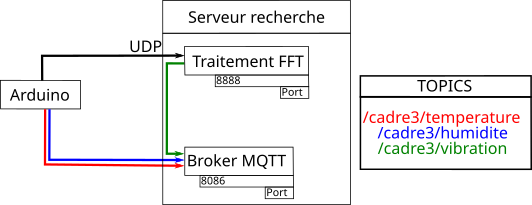
\includegraphics[scale=1]{../img/schemaNet.png}
	\captionof{figure}{Schema Réseaux}
    \label{SN}
\end{center}
\subsubsection{Liaisons MQTT}
Afin d'envoyer les données du microcontroleur vers le serveur j'ai choisi le protocle MQTT et ce pour deux raisons.La premier est que le projet seras amener à évoluer et contiendras plusieurs capteur récoltant la même données à des endroits different de la ruche. Ainsi avec le systéme de topics, on pouras identifier facilement ces différent capteur. La deuxième est que la solution envisager pour le site web, et la base de données, est trés facilement couplabe avec ce protocole. 

\begin{scriptsize}
\begin{lstlisting}


\end{lstlisting}
\end{scriptsize}

\subsubsection{Liaisons UDP}

\begin{scriptsize}
\begin{lstlisting}

void gatherVibration(char * fdata, int nbEchantillon, int nbVirgule, double periodeEchantillonageMs)
{
	// Afin d'avoire le nombre de caractere je fait le nombre de chiffre apres la virgule plus deux
	// qui represente mon premier digits et ma virgule.
	int nbChar = nbVirgule+2;
	char tmp[nbEchantillon][nbChar];
	char data2[nbEchantillon*nbChar];
	double centsValeurs[nbEchantillon];
	int i,y;
	for(i=0;i<nbEchantillon;i++){
		centsValeurs[i]=analogRead(piezo);
		centsValeurs[i]=(centsValeurs[i]*5)/1023;
		delay(periodeEchantillonageMs);
	}
	delay(2000);
	for(i=0;i<nbEchantillon;i++){
		dtostrf(centsValeurs[i],nbChar,nbVirgule,tmp[i]);
		for(y=0;y<nbChar;y++){
			data2[(nbChar*i)+y]=tmp[i][y];
		}	
	}
	Serial.println(data2);
	Udp.beginPacket(ipUdp,PORT_UDP);
	Udp.write(data2);
	Udp.endPacket();
}

\end{lstlisting}
\end{scriptsize}

\section{Conclusion}

\newpage
\listoffigures

\end{document}
